\section{1965: Minicomputers and Time-sharing System}
In the shadow of the large main frame monsters a new generation of computers
emerged around 1965: Mini computers. The first was the PDP-1 of DEC (Digital
Equipment Corp.), later to be followed by the very popular PDP-8. They were
mounted on standard 19" racks for typical use in laboratories, and they were built
with discrete bipolar junction transistors and magnetic core memories. Their word-
length was 18 bits (PDP-1), 12 bits (PDP-8) and 16 bits (HP 2116). Their cycle
time lay around 2 us. Every instruction needed 1 or 2 cycles. For the time, this was
considered very fast. Their instruction sets contained load and store instructions,
logical operations, single-bit shifts, and add and subtract. Multiplication and
division was to be programmed. Their memory sizes being small, typically 4K or 8K
words, compilers for high-level languages were out of the question. They were
connected to a typewriter (teletype) for input and output.

The minicomputers' distinct attraction was their direct accessibility. They were not
hidden in computation centers, but allowed interactive use. The old scheme of
sign-up hours had returned which, inherently, is inefficient.

As an example, we sketch the structure of the popular PDP-8. Its memory
consisted of magnetic cores, 4096 words, 12 bits long. The computational unit
contained the accumulator, also 12 bits long. Instructions came in (essentially) two
variants. Memory reference instructions and operators in micro-instruction format.
\begin{figure}[h!]
  \centering
  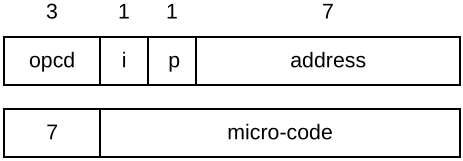
\includegraphics[width=.75\textwidth]{i/3}
  \caption{i=indirection, p=mem page}
\end{figure}

The memory reference instructions include loading, storing, adding, logical and,
and jumps. This description makes it clear that such minicomputers were apt to be
coded "by hand" with the aid of an assembler. Compilers were out of the question;
the resulting code would be too long and inefficient. The memory was small
enough to ensure that only small programs could be loaded, typically for controlling
equipment and data acquisition.

A most remarkable novelty was the first time-sharing system with the goal of
allowing fully interactive use without monopolizing the computer. This system was
developed by Dennis and van Horn at MIT. In cooperation with DEC they devised
an augmented PDP-1. It was beefed up by a drum store with 16 tracks of 4K words
in each. Furthermore, the main store was enlarged to 3 blocks of 4K words. The
first section was used for a small "operating system" .The system allowed 16
programmers to work on the single computer quasi-simultaneously. It operated in
time slices of 33 ms duration. In every slice, three actions occurred: A track was
read alternately from the drum into main store section 2 (or 3) , the same main
store section was dumped onto the appropriate drum track, and the processor
executed the program in main store section 3 (or 2). This allowed every
programmer to obtain the impression that a regular PDP-1 was at his exclusive
disposal. The scheduling of the processor, i.e. its allocation to an individual user,
was quite simple. Users being statically given a place in a ring, the next time-slice
was given to the next user in the ring, except, if he was waiting for input or output.
\begin{figure}[h!]
  \centering
  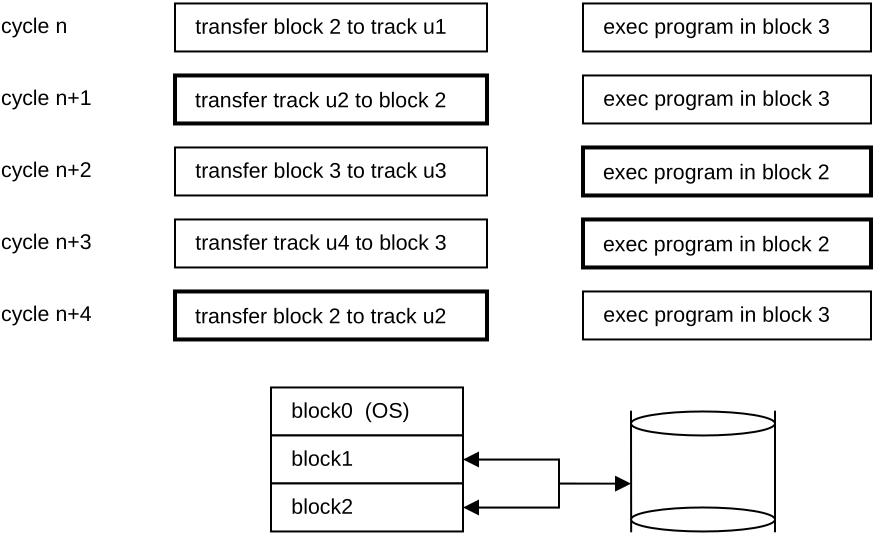
\includegraphics[width=\textwidth]{i/4}
\end{figure}

Probably the first such system was installed at Stanford University in 1964 in an
experimental lab for teaching programming (Prof. Suppes). In order to facilitate
textual input and control features, a special key was included in the keyboard of
each station. It later became ubiquitous and called the CTRL-key.

This idea of time-sharing was simple and fascinating. Soon such systems became
a normality. Manufacturers of main frames caught on to the idea and extended
their products accordingly (IBM 360/67, GE 645). But they believed that software
was omnipotent, and did not restrict themselves to a fixed time slice scheme, nor
to fixed memory allocation for every user. Individual, dynamic resource allocation
was their vision, memory sizes according to every user's needs, and scheduling
individually according to priorities and resource availability. A side-effect was the
emergence of memory management units in the hardware of these multi-user
computers. This was pioneered by the giant Atlas computer in Manchester.

These were high-flying goals. Nobody had ever designed systems of this
complexity. The difficulties had been vastly underestimated, Yet, delivery times
had been promised to eager customers. The dire situation was met by employing
huge crowds of system programmers, resulting in overwhelming management and
communication problems. It ended in what was (in 1968) called the software crisis,
documented very aptly by Fred Brooks’ book \emph{The mythical man month}, culminating
in the wise insight that "adding man power to a late project makes it later".

Compilers together with OS/3860 became what was (perhaps) the first of the
software giants, systems that did not rest on coherent design elements, built by
armies of programmers, and in their entirety understood by nobody, and as a result
of questionable reliability. Failures had been pre-programmed. Updates became a
monthly routine.

Software, that is operating system, compilers, and libraries, were delivered by the
computer manufacturers like an accessory. As software grew to huge dimensions
and generated large cost, the process of "unbundling" started. Software became
an object of its own, and its pricing was separated from that of hardware. This
occurred not without intervention from legal courts. Software companies emerged.
They generated programs usable on many different brands of computers and
founded a market of its own.
